\begin{frame}
  \frametitle{$h$-Adaptivity (small $\kappa$ case)}
  \begin{itemize}
    \item{We now employ an extremely simple flux jump error estimator to drive adaptivity
  \begin{equation}
    \nonumber
    \eta^{\text{FLUX}}_K := \left( {h_K} \int_{\partial K} |R_K|^2 ds \right)^{1/2}
    \label{eqn:flux_indicator}
  \end{equation}
  }

    \item{
where $R_K$ is the local residual defined by
\begin{equation}
  \nonumber
  R_K := \left\{
    \begin{array}{cl}
      0, & s \in \partial K \cap \Gamma_D \\
      g_N - \nabla u_h \cdot n_K, & s \in \partial K \cap \Gamma_N \\
      \frac{1}{2}(\nabla u_h|_L - \nabla u_h|_K) \cdot n_K, & s \in \partial K \cap \partial L \neq \emptyset
    \end{array}
    \right.
  \label{eqn:residual}
\end{equation}
%% where $g_N$ is given Neumann boundary data, $n_K$ is the outward unit
%% normal for cell $K$, and cell $L$ shares an edge (face) with cell $K$
%% in the finite element mesh.
}
  \end{itemize}
\end{frame}


\begin{frame}
  \frametitle{Biquadratic Adaptivity}
  \begin{center}
	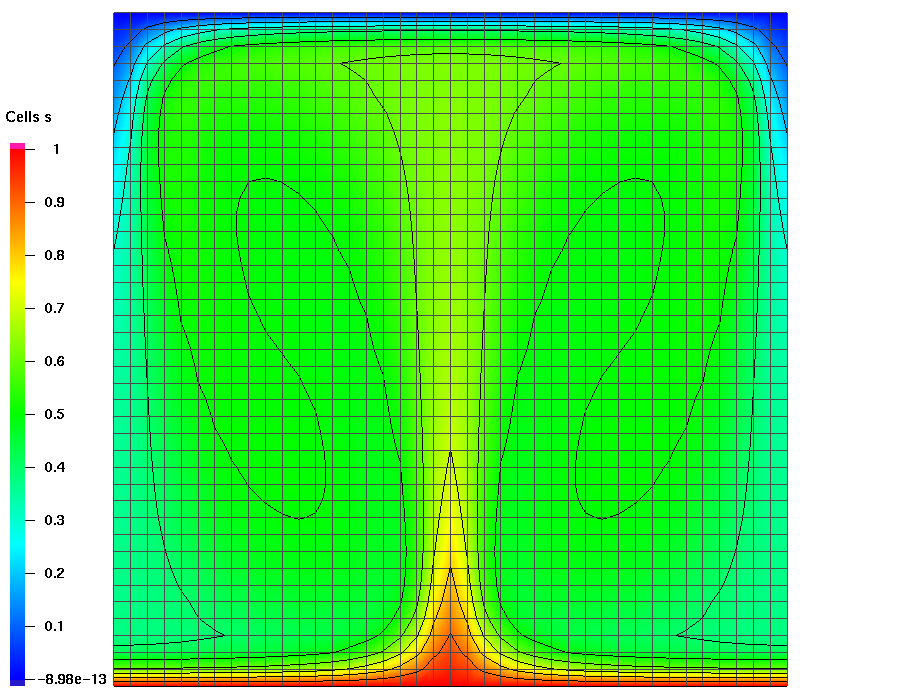
\includegraphics[width=.8\textwidth]{figures/biquad_amr_0000}    
  \end{center}
\end{frame}
  
\begin{frame}
  \frametitle{Biquadratic Adaptivity}
  \begin{center}
	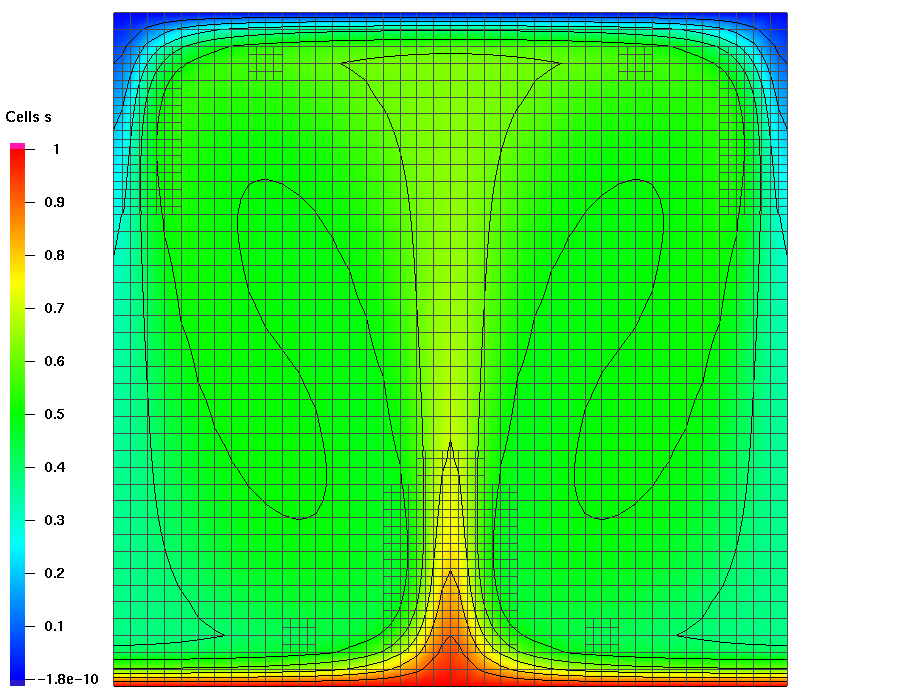
\includegraphics[width=.8\textwidth]{figures/biquad_amr_0001}    
  \end{center}
\end{frame}

  \begin{frame}
  \frametitle{Biquadratic Adaptivity}
  \begin{center}
	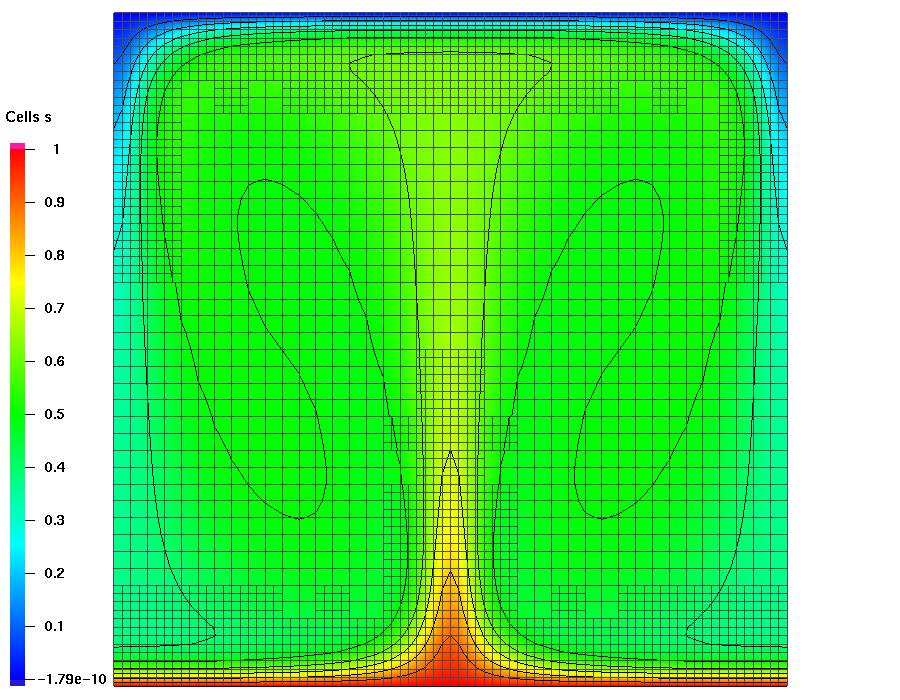
\includegraphics[width=.8\textwidth]{figures/biquad_amr_0002}    
  \end{center}
\end{frame}
\begin{frame}
  \frametitle{Biquadratic Adaptivity}
  \begin{center}
	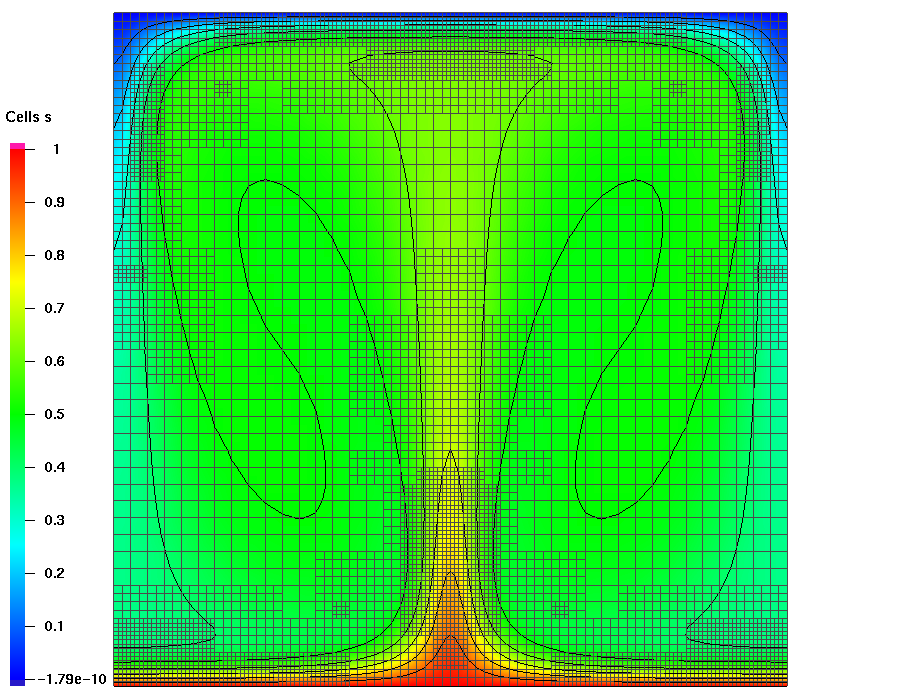
\includegraphics[width=.8\textwidth]{figures/biquad_amr_0003}    
  \end{center}
\end{frame}
\begin{frame}
  \frametitle{Biquadratic Adaptivity}
  \begin{center}
	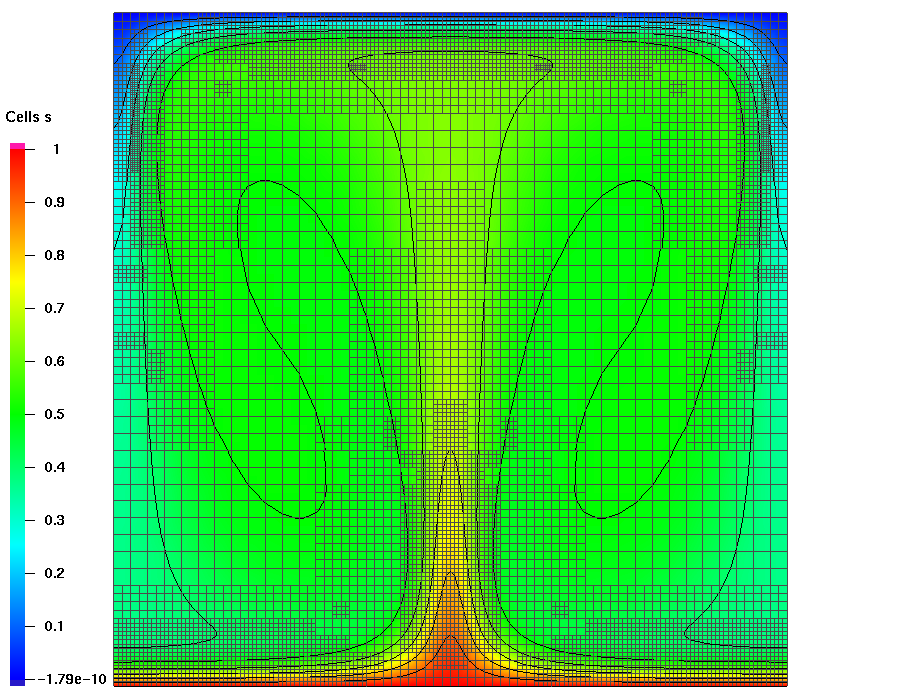
\includegraphics[width=.8\textwidth]{figures/biquad_amr_0004}    
  \end{center}
\end{frame}
\begin{frame}
  \frametitle{Biquadratic Adaptivity}
  \begin{center}
	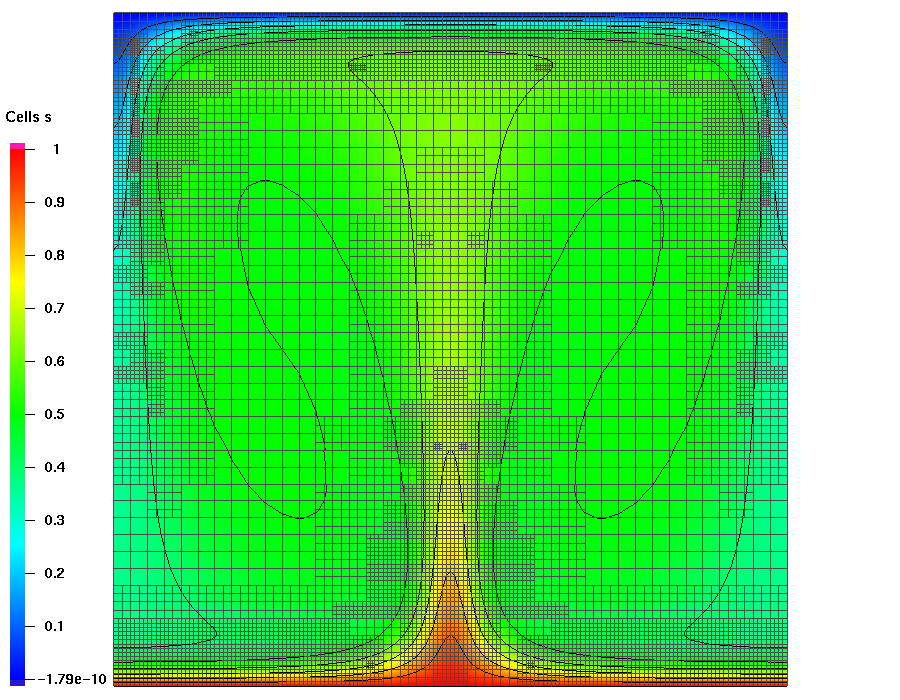
\includegraphics[width=.8\textwidth]{figures/biquad_amr_0005}    
  \end{center}
\end{frame}
\begin{frame}
  \frametitle{Biquadratic Adaptivity}
  \begin{center}
	\includegraphics[width=.9\textwidth]{figures/biquad_adapt_vs_unif_thermal}    
  \end{center}
\end{frame}
\begin{frame}
  \frametitle{Biquadratic Adaptivity}
  \begin{center}
	\includegraphics[width=.9\textwidth]{figures/biquad_adapt_vs_unif_solute}    
  \end{center}
\end{frame}






\begin{frame}
  \frametitle{Future Work}
  \begin{itemize}
    \item{Improved (practical) error indicators}
    \item{Explain higher-than-expected accuracy of classical
      flux calculation for bilinear elements} 
  \end{itemize}
\end{frame}
